\section{Introduction}
In this section we are going to present some of the recent work and research that was done regarding skin cancer detection and classification using machine learning , we are going to explore the various methods, tools, new ideas and challenges that was handeled by researchers for the hope of getting a clear understanding of the problem and how to go about solving it depending on each one's conditions, requirements and goals.



\section{skin cancer detection and classification using machine learning}
\begin{description}
    \item [proposed methodology]
    the proposed methodology in this article ~\cite{Krishna2020} uses a 6 step process (input data - preprocessing - segmentation - feature extraction - classification - output data)
    \item [input data] 
        dermoscopic images from the ISIC ( International Skin Imaging Collaboration) 2019 challenge containing 8 classes of skin cancer, and for simplisity reasons only 800 images out of 25000 is used.
    
    \item [preprocessing]
        because of the heteroginity of the input data a preprocessing step is required to inhance the quality of images and remove irrelevant parts. the main technices used here are gray scale conversion and the application of the Gaussian and median filter for noise removal and enhancement, and for the unwanted hair they applied the Dull Razor method (a preprocessing algorithm), as shown in figure ~\ref{fig:Preprocessing}

    \item [segmentation]
        segmnetation is used to extract the region of interest and for that they used a k-means clustering algorithm as shown in figure \ref{fig:segmentation}
        
    \item [feature extraction]
        for this they used 2 well know methods, ABCD method and GLCM. ABCD is used in dermatological applications and diagnosis for skin lesions such as melanomas and it is the abreviation of Asymmetry, Border, Color and Diameter. Grey Level Co-occurrence Matrix (GLCM) is used for texture analysis, other features are also used in addition to these 2 methods for further classification such as Autocorrelation, correlation, Standard vector...etc
    
    \item [classification]
        for classification they used MSVM (Multi-class Support vector machine) machine learning algorithm, they used trainning and testing ratios of 70:30 and obtained an acuuracy of 96.25\% and the confusion matrix shown in figure \ref{fig:confusion-matrix}
\end{description}

\begin{figure}[htbp]
\begin{center}
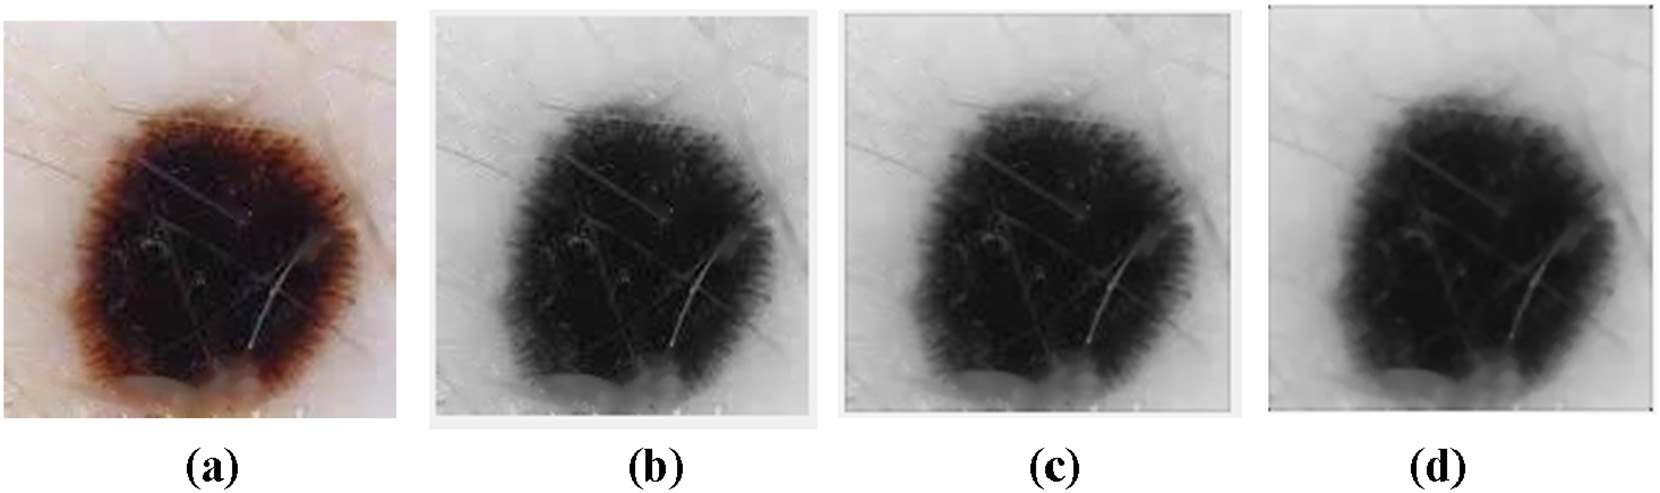
\includegraphics[width=15cm]{./chapter-03-state-of-the-art/preprocessing.png}
\end{center}
\caption{Preprocessing: (a)Dull razor image, (b) Gray scale image, (c) Gaussian filter, (d) Median filter.}
\label{fig:Preprocessing}
\end{figure}




\begin{figure}[htbp]
\begin{center}
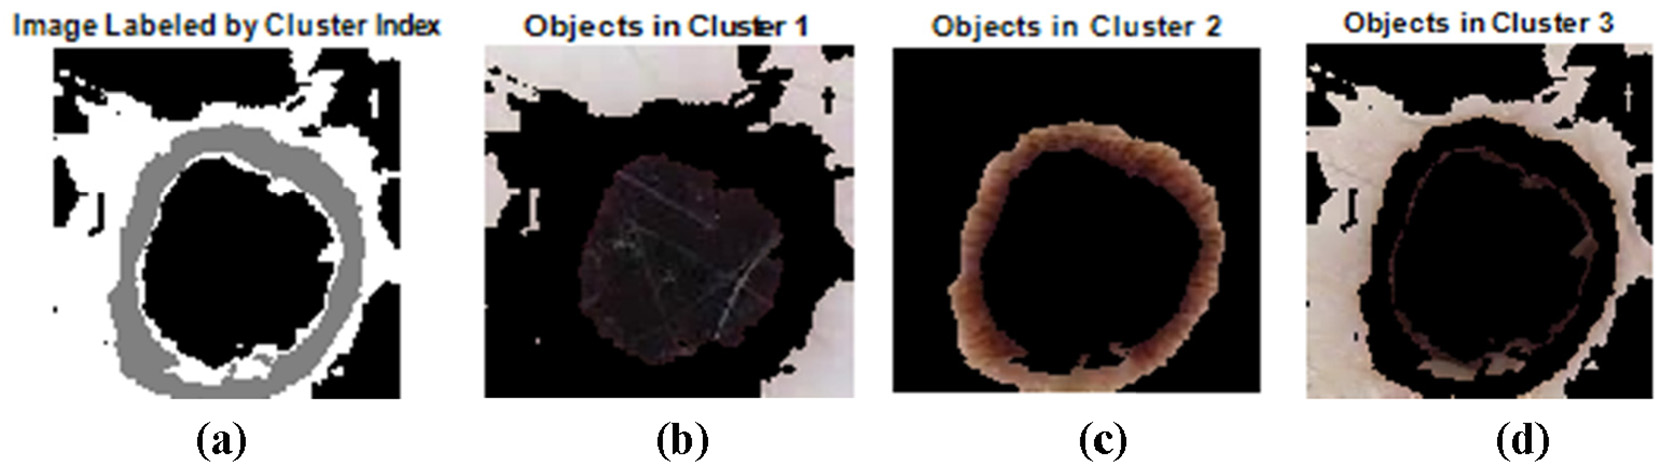
\includegraphics[width=15cm]{./chapter-03-state-of-the-art/segmentation.png}
\end{center}
\caption{Segmentation: (a) Image labelled by cluster index, (b) Objects in cluster 1, (c) Objects in cluster 2, (d) Objects in cluster 3.}
\label{fig:segmentation}
\end{figure}


\begin{figure}[htbp]
\begin{center}
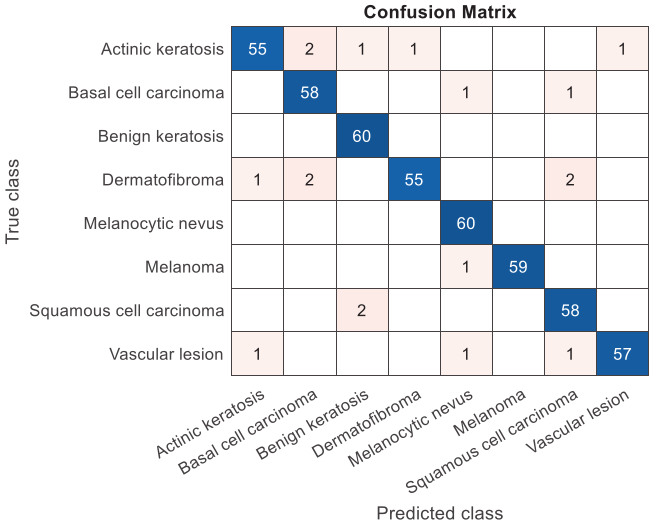
\includegraphics[width=15cm]{./chapter-03-state-of-the-art/confusion-matrix.png}
\end{center}
\caption{Confusion Matrix}
\label{fig:confusion-matrix}
\end{figure}


% \begin{figure}[htbp]
% \begin{center}
% 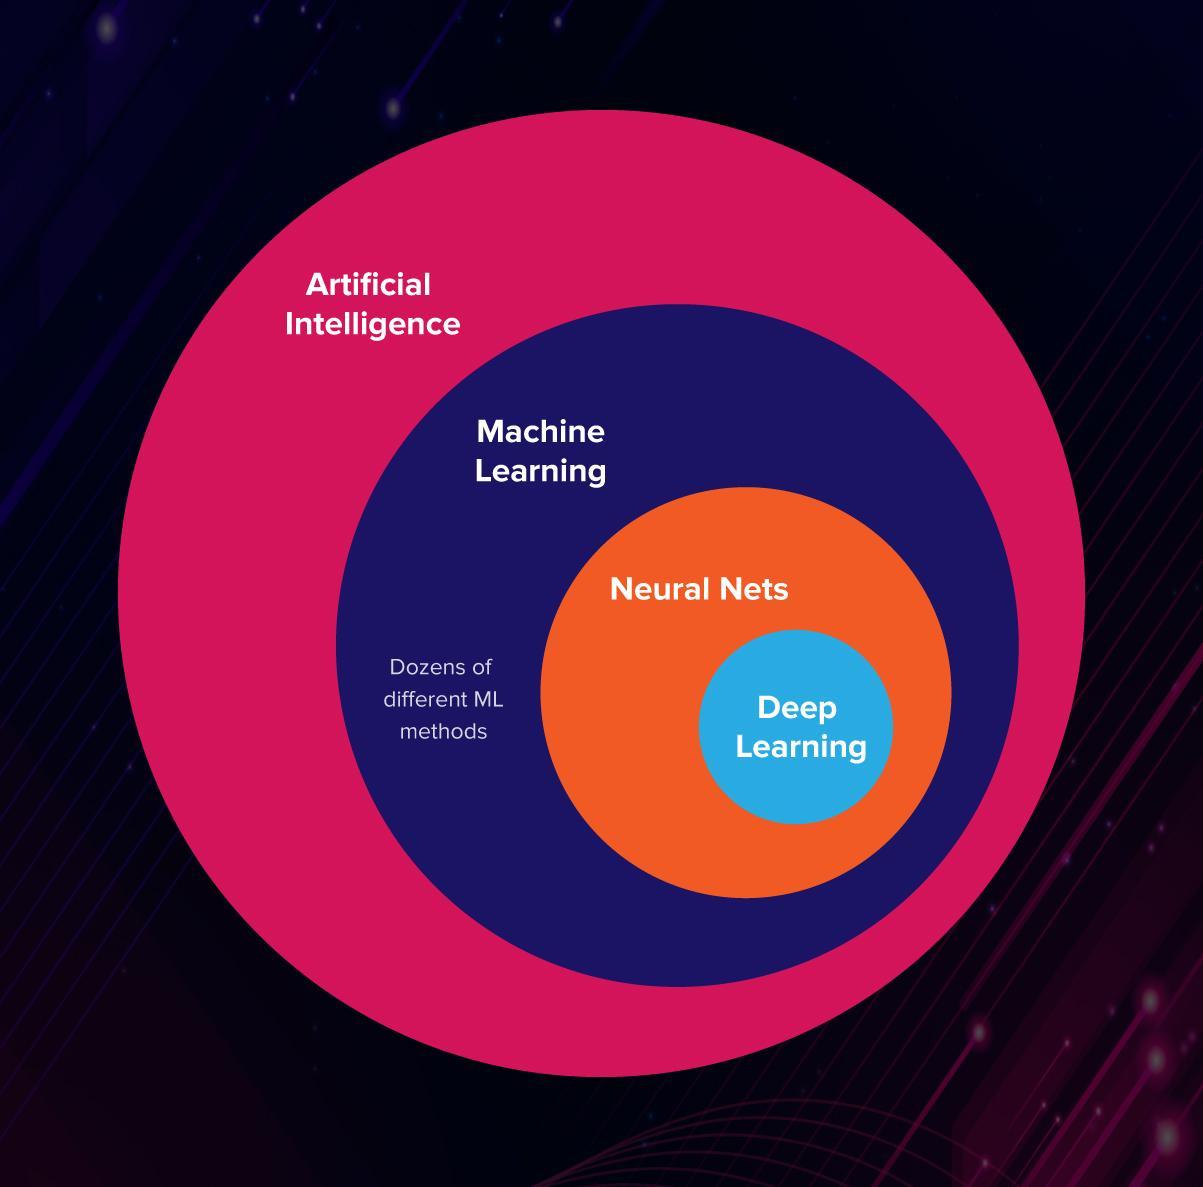
\includegraphics[width=2cm]{./chapter-03-state-of-the-art/versus.jpg}
% \end{center}
% \caption{}
% \label{fig:}
% \end{figure}
